\chapter{Annexes}

\lstset{ 
    basicstyle=\ttfamily\small,
    breaklines=true, 
    frame=single, 
    xleftmargin=20pt,
    xrightmargin=20pt, 
}

\section{Références bibliographiques}


    \begin{itemize}
        \item $\bullet$ \url{https://cdn.bodanius.com/media/1/a9c1593_fiche-technique-du-tcrt5000.pdf} pour les capteurs de positions 
        \item $\bullet$ \url{https://www.adeept.com/ultrasonic-sr04_p0047.html} pour le capteur a ultrason (récupération de la tension et du courant d'entrée necessaire pour déterminer la puissance)
        \item $\bullet$ \url{https://cdn.bodanius.com/media/1/8c2164078_l293d.pdf} pour les bouclier thermiques (carte moteur)
        \item $\bullet$ \url{https://www.openhacks.com/uploadsproductos/eone-1602a1.pdf} pour l'écran LCD et le controleur de l'écran (référence dans le tableau section: 3.0ELECTRICAL CHARACTERISTICS)
        \item $\bullet$ \url{https://moodle.insa-rouen.fr/pluginfile.php/184607/mod_resource/content/5/Lab_Sheet__1.pdf} pour la LED suivis de 
        \item $\bullet$ \url{https://www.adeept.com/4pcsled_p0104.html} pour la la LED (documentation et informations manquantes pour le sujet, on utilise donc le cas général pour une led rouge)
        \item $\bullet$ \url{https://www.adeept.com/passivebuzzer_p0284.html} pour le buzzer, la documentation est manquante, on prendra la cas "général" de la consomation énergétique d'un buzzer. 
        \item $\bullet$ \url{https://www.adeept.com/2xn20-with-holder_p0335.html} pour les moteurs, consommation maximale en ampère prise en compte.         
        \item $\bullet$ \url{https://moodle.insa-rouen.fr/pluginfile.php/31526/mod_label/intro/documentation.pdf} pour la documentation Latex
        
    \end{itemize}

\newpage
\section{Glossaire}
    \begin{table}[ht]
        \begin{adjustwidth}{-3cm}{-3cm}
            \centering
            \begin{tabular}{|p{1cm}|p{5cm}|p{10cm}|}
                \hline
                \textbf{Nom} & \textbf{abréviation} & \textbf{Définition}\\
                \hline
                TAD & Type Abstrait de Données & Structure de données définie par des opérations (est indépendant du language de programmation).\\
                \hline
                GPIO & General Purpose Input/Output & Une broche de la carte Raspberry qui peut être configurée comme une entée pour reçevoir un signal ou comme une sortie pour reçevoir un signal.\\ 
                \hline
                SDA & Serial Data Line & Ligne de commmunication utilisé dans les bus I2C utilisée pour envoyer et reçevoir des données.\\
                \hline
                SCL & Serial Clock Line & Ligne de communication utilisé dans les bus I2C utilisée pour synchoniser la transmition de données (définit l'orloge).\\
                \hline
                I2C & Inter-Integrated Circuit & Protocole de communication entre composants.\\
                \hline
                GND & Ground & Masse du circuit électronique.\\
                \hline
                VCC & Voltage at the Common Collector & Source de tension positive d'alimentation d'un circuit électronique.\\
                \hline
                Trig & Trigger & Ligne utilisée pour le signal de déclanchement d'un capteur.\\
                \hline
                Tx & Transmit & Ligne utilisée pour la transmition de données.\\
                \hline
                Rx & Receive & Ligne utilisée pour la réception de données.\\
                \hline
                Echo & écho & Signal reçu du capteur à ultrason après réverbération du son sur une surface.\\
                \hline
                LED & Light Emitting Diode & Composant électronique qui emmet de la lumière lorsque un certain seuil de tension est dépassé (consomme moins d'électricité qu'une lampe classique).\\
                \hline
                PWM & Pulse Width Modulation & Le signal envoyé peut changer la durée des impulsions. \\     
                \hline
                SD & Secure Digital & carte mémoire pour stocker des données. \\
                \hline
                SSH & Secure Shell & Protocole de communication crypté pour se connexter à distance sur un autre appareil.\\
                \hline
                RAM & Random Acces Memory & Mémoire en accès direct, stocke temporairement des données.\\
                \hline
                EN & Enable & Ligne utilisée pour activer ou désactiver un circuit électronique.\\
                \hline
                LCD & Liquid Crystal Display & Permet de crontrôler la quantité de lumière qui passe à travers de l'écran à l'aide d'un champ électrique.\\
                \hline
            \end{tabular}
        \end{adjustwidth}
    \end{table}


\section{Analyses descendente version PDF} 
    Ci dessous sont présentés en format page entière les analyses descendantes mises en place lors du cycle en V.
    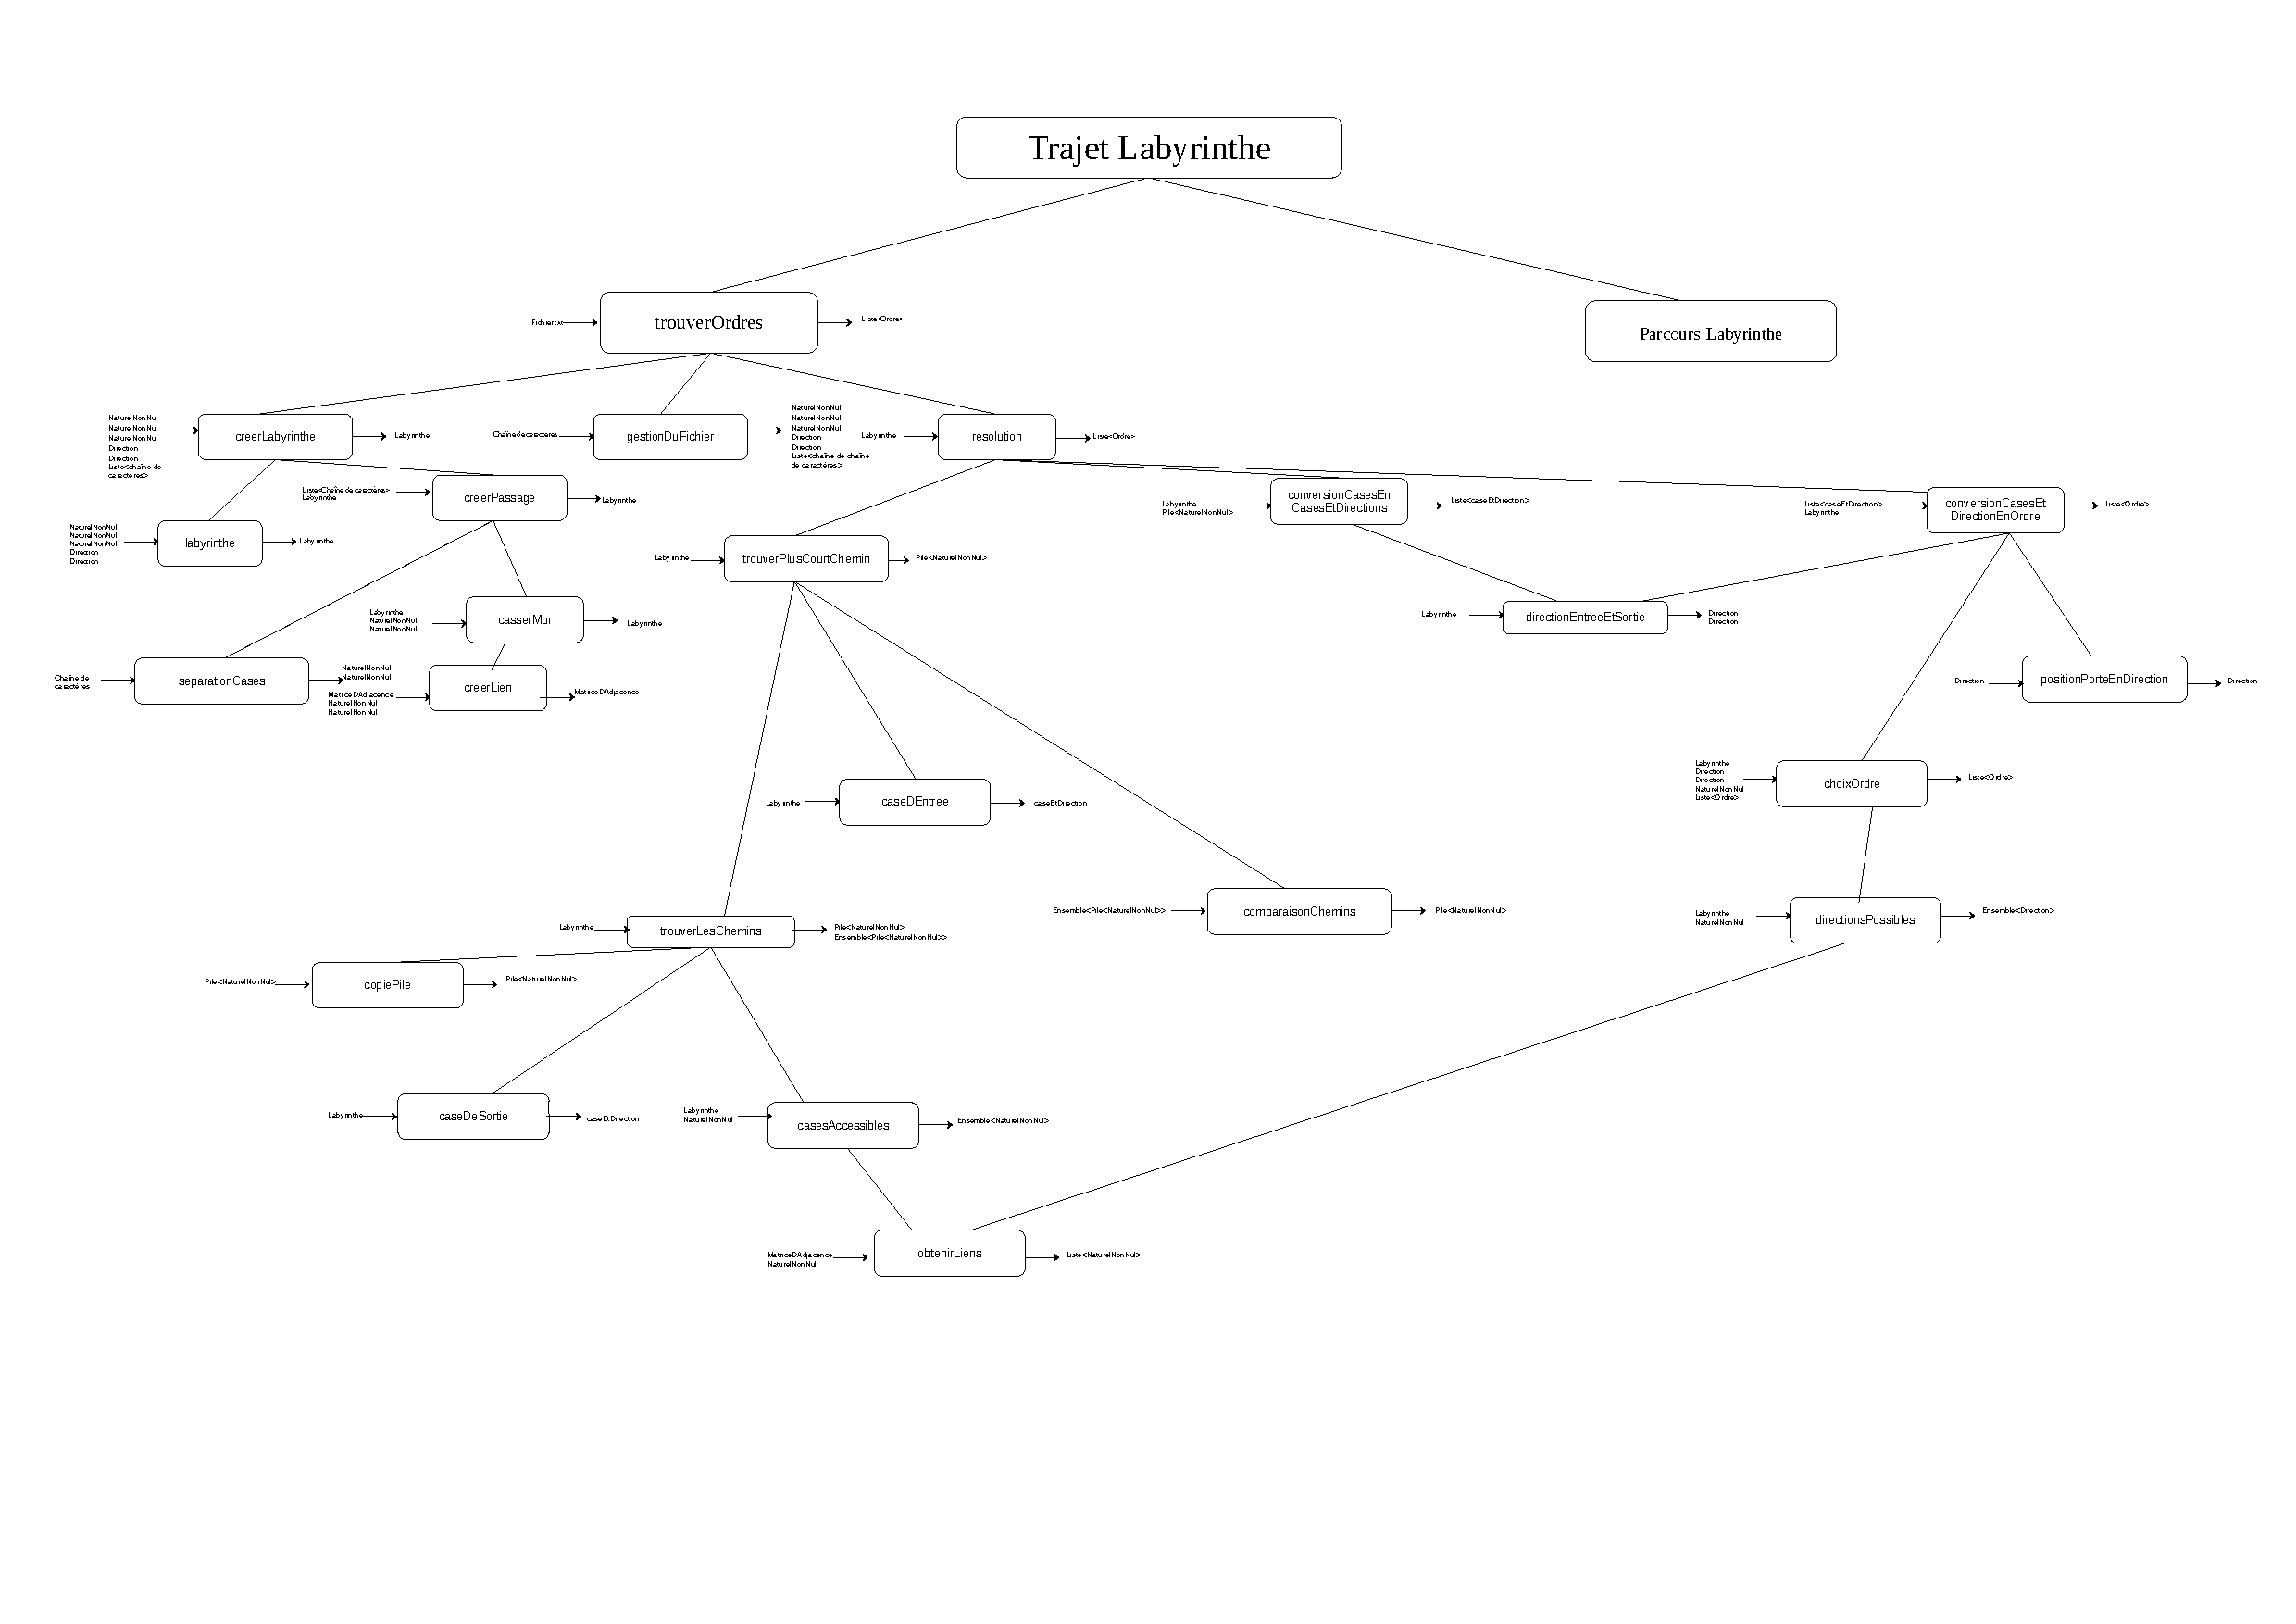
\includepdf[pages=-]{algo/analyse/analyseDescendante_Algo.pdf} 
    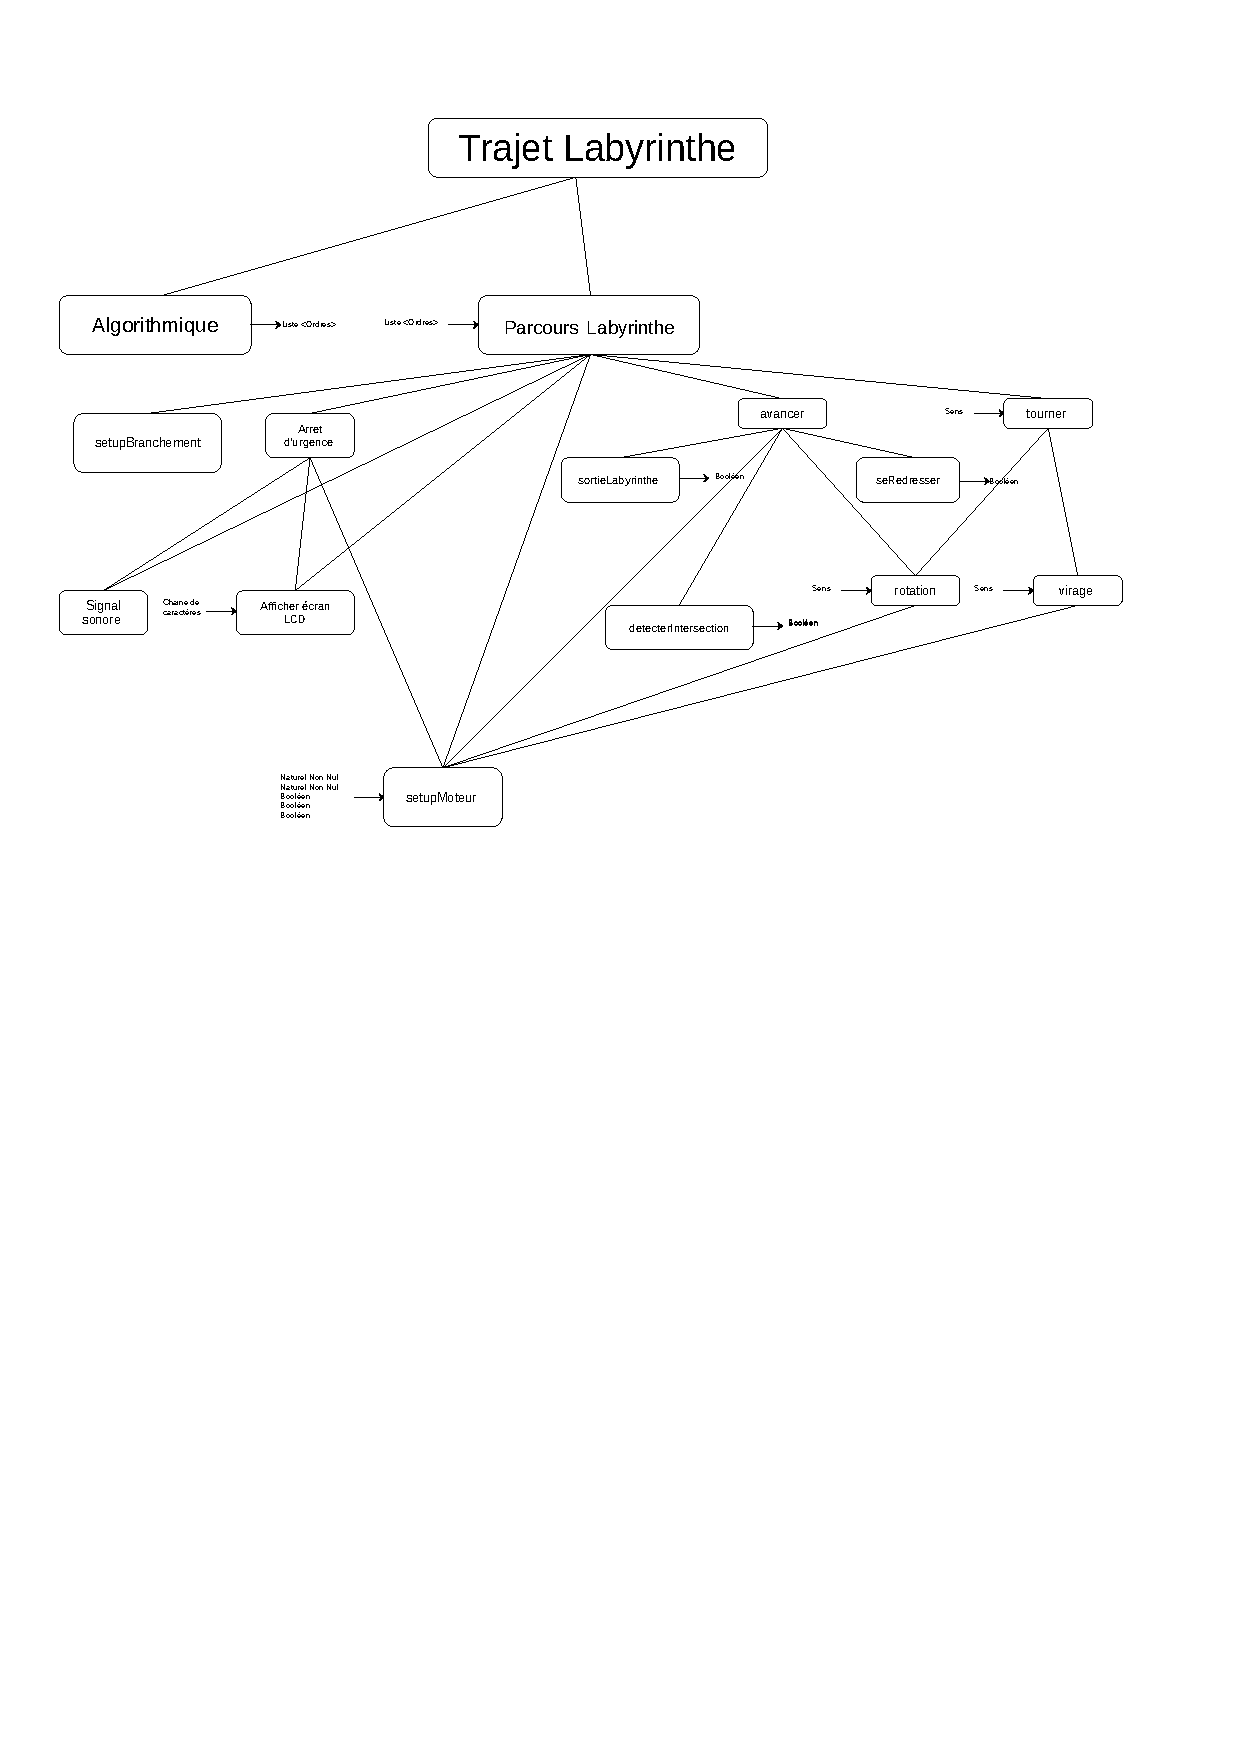
\includepdf[pages=-]{elec/analyseDescendante_Elec.pdf} 

\section{Fichiers .c}

    \subsection{Les Types}
        \subsubsection{Les listes}
            \lstinputlisting[language=C]{../Programme/src/Types/ListeDeNNN.c}
            \lstinputlisting[language=C]{../Programme/src/Types/ListeDOrdre.c}
            \lstinputlisting[language=C]{../Programme/src/Types/ListeDeCDC.c}
            \lstinputlisting[language=C]{../Programme/src/Types/ListeDeCaseEtDirection.c}

        \subsubsection{Les listes chaînées}
            \lstinputlisting[language=C]{../Programme/src/Types/ListeChaineeDeNNN.c}
            \lstinputlisting[language=C]{../Programme/src/Types/ListeChaineeDOrdre.c}
            \lstinputlisting[language=C]{../Programme/src/Types/ListeChaineeDeCDC.c}
            \lstinputlisting[language=C]{../Programme/src/Types/ListeChaineeDeCaseEtDirection.c}
            \lstinputlisting[language=C]{../Programme/src/Types/ListeChaineeDeDirection.c}
            \lstinputlisting[language=C]{../Programme/src/Types/ListeChaineeDePileDeNNN.c}

        \subsubsection{Les ensembles}
            \lstinputlisting[language=C]{../Programme/src/Types/EnsembleDeNNN.c}
            \lstinputlisting[language=C]{../Programme/src/Types/EnsembleDeDirection.c}
            \lstinputlisting[language=C]{../Programme/src/Types/EnsembleDePileDeNNN.c}

        \subsubsection{Les autres types}
            \lstinputlisting[language=C]{../Programme/src/Types/PileDeNNN.c}
            \lstinputlisting[language=C]{../Programme/src/Types/MatriceDAdjacence.c}
            \lstinputlisting[language=C]{../Programme/src/Types/Ordre.c}
            \lstinputlisting[language=C]{../Programme/src/Types/caseEtDirection.c}
            \lstinputlisting[language=C]{../Programme/src/Types/Direction.c}
            \lstinputlisting[language=C]{../Programme/src/Types/labyrinthe.c}



